The \verb?Snd_Driver? module is an audio signal coder/decoder. It translates the signal between a parallel format and a bit serial format. The parallel format is sent to the \verb?Vol_Bal? module which processes the sound and sends it to the class-D amplifier. The bit serial format is used by the WM8731 chip and the amplifier. This module will be a complete copy of the module used in \emph{Laboration 4}. In this case the module \verb?Vol_Bal? will replace and expand the \verb?Application? used in that laboration.

\begin{figure}[H]
  \centering
  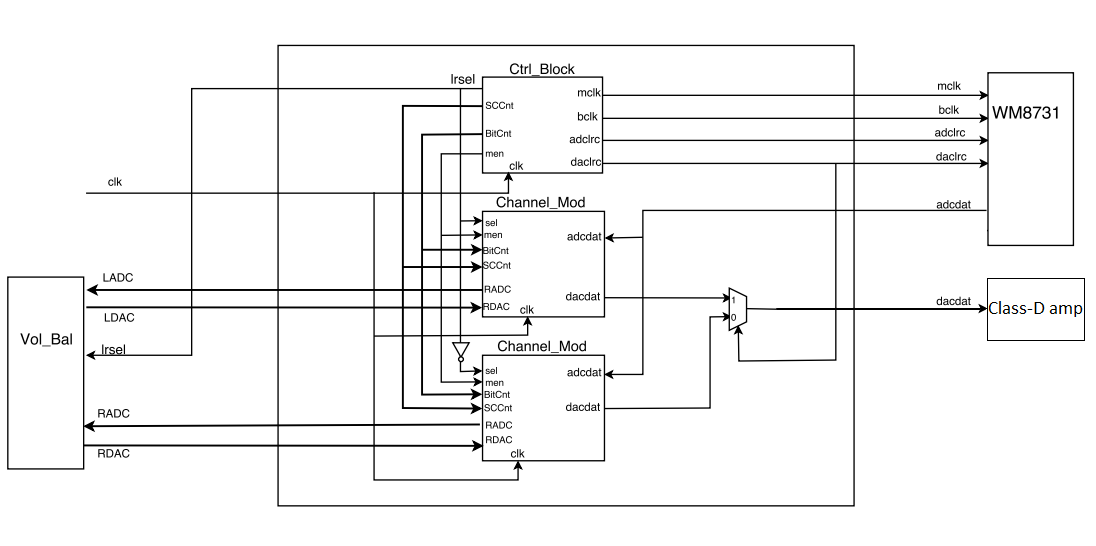
\includegraphics[scale=.40]{snddriver}
  \caption{The \texttt{Snd\_Driver} schematic, as seen in Lab 4, Audio Codec.}
  \label{fig:sndDriver}
\end{figure}
